In the most basic sense, all neural network operators need to be able to take in a set of numbers and perform calculations on them, then provide an output.
The shape can change from input to output, depending on the operator.
Some operators, like the \emph{perceptron} (or its conceptual successors, the \emph{fcl} and \emph{MLP}) have trainable weights that get updated like described in \autoref{sec:theory-neuralnetworktraining}.
Others, like the \emph{pooling operator} transform the data according to static rules, without trainable parameters.
A neural network can't be trained, if it doesn't contain operators with adjustable weights.
However operators like pooling are very efficient in supporting trainable operators (as will be shown later).

\paragraph{The perceptron} is the most basic building block of all neural network architectures.
A schematic view is given in \autoref{fig:perceptron}.

\begin{figure}[htbp]
    \centering
    \makebox[\textwidth][c]{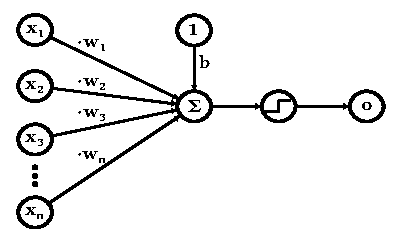
\includegraphics[width=0.6\textwidth]{./architectures/theory/perceptron-pooling/perceptron.pdf}}
    \caption{Schematic representation of a perceptron. Inputs are denoted with $x_i$, weights with $w_i$, the bias value with $b$ and the output with $o$. 
        The inputs get scaled with the weights, summed and the bias is added.
        Then the value is passed through a not specified non-linear function (e.g. ReLU or the sigmoid function).
    }
    \label{fig:perceptron}
\end{figure}

The output gets calculated like $o = \mathrm{ReLU} \left(\sum\limits_{i=1}^{n} x_i\cdot w_i + b\right)$.
Calculating multiple perceptrons with different weights in parallel for the same input values $x$ is called a fully connected layer (fcl).
The formula for the elements in a fcl is show in \autoref{eq:fcl},

\begin{equation}
    \label{eq:fcl} 
    o_j = \sum\limits_{i=1}^{n} x_i\cdot w_{i, j} + b_j
\end{equation}

which is equivalent to a matrix-vector-multiplication. Therefore the fcl can be evaluated quickly.
\autoref{fig:image-classification-general} shows multiple fcls in series, which is called a multi layer perceptron (MLP). 

\paragraph{The pooling operator} is basically a function that selects a new value based on values in a specific range around the target position.
The rules can range from taking the \emph{minimal} value, to the \emph{maximum} value or the \emph{average}.
In this thesis, all pooling operations are average pooling.

\begin{figure}[htbp]
    \centering
    \makebox[\textwidth][c]{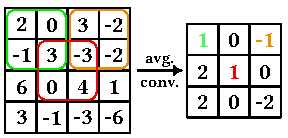
\includegraphics[width=0.6\textwidth]{./architectures/theory/perceptron-pooling/pooling.pdf}}
    \vspace{-0.2cm}
    \caption{
        Example for a 2$\times$2-average-pooling operation. The colors indicate what numbers get averaged. 
        Not all blocks are colored, but the calculation is performed analogously.
    }
    \label{fig:pooling}
\end{figure}

\autoref{fig:pooling} shows an example of an 2$\times$2-average-pooling operation.
Where the dimension of input and output need to stay the same, the border of the input is padded with zero values (no padding in this example).